\documentclass[12pt, a4paper]{report}
\usepackage[top=3cm,left=3cm,right=2cm,bottom=2cm]{geometry}
\linespread{1.3}
\setlength{\parindent}{1.25cm}
\usepackage{indentfirst}
\usepackage[utf8]{inputenc}
\usepackage[brazil]{babel}
\usepackage{amsmath}
\usepackage{amsthm}
\usepackage{amsfonts}
\usepackage{amssymb}
\usepackage{graphicx}
\usepackage{color}
\usepackage{multicol}
\usepackage[normalem]{ulem}
\usepackage{wrapfig}
\usepackage{caption}
\usepackage{fancybox}
\usepackage[pdfstartview=FitH]{hyperref}
\usepackage{subfigure}
\bibliographystyle{plain}
\usepackage{algorithm}
\usepackage{algpseudocode}
\usepackage{float}


\graphicspath{{Figuras/}}

\renewcommand{\theenumii}{\alph{enumii}}
\DeclareMathOperator{\sen}{sen}
\DeclareMathOperator{\tg}{tg}
\DeclareMathOperator{\arctg}{arctg}
\DeclareMathOperator{\cotg}{cotg}
\DeclareMathOperator{\agm}{agm}

\newtheorem{thm}{Teorema}[section]
\newtheorem{dfn}{Definição}[section]
\newtheorem{prob}{Problema}[section]
\newtheorem{cor}{Corolário}[section]
\newtheorem{prop}{Proposição}[section]
\newtheorem{lem}{Lema} [section]

\newcounter{contar}
%  #endregion preâmbulo

% #region Variáveis 
\newcommand{\nomeUniversidade}{Universidade Federal da Bahia}
\newcommand{\nomeInstituto}{Instituto de Computação}
\newcommand{\nomeCurso}{MATA53 - Teoria dos grafos}
\newcommand{\nomeProfessor}{Islame Felipe da Costa Fernandes}
\newcommand{\nomeGrupo}{\sc{\large{Antoniel Magalhães}} \\
\sc{\large{João Leahy}} \\
\sc{\large{Luis Felipe}}}
\newcommand{\titulo}{\sc{\Large{Problema de Colocação Ótima de Câmeras de Segurança no bairro da Ondina}}}
% #endregion Variáveis 

\begin{document}

% #region capa
\pagestyle{empty}
\begin{center}

\includegraphics[height=2.5cm]{UFBA.jpg}
\hspace{2cm}
\end{center}

\begin{center}
\sc{\large{\nomeUniversidade}} \\
\sc{\large{\nomeInstituto}} \\
\sc{\small{\nomeCurso}} \\

\vspace{4cm}

\titulo

\vspace{4.5cm}

\nomeGrupo


\vspace{5.5cm}

\textbf{Salvador - Bahia} \\
\today
\end{center}
% #endregion capa

% #region folha de rosto
\newpage
\begin{center}
\titulo

\vspace{4cm}

\nomeGrupo
\end{center}

\vspace{4cm}

\begin{flushright}
\begin{minipage}{8.6cm}
Projeto final entregue ao professor \nomeProfessor\ 
como método avaliativo da disciplina \nomeCurso


\end{minipage}
\end{flushright}
 
\vspace{8cm}


\begin{center}
\textbf{Salvador - Bahia} \\
\today
\end{center}

% #endregion folha de rosto

% #region Índice
\newpage
\tableofcontents
\thispagestyle{empty}
\newpage
\setcounter{page}{1}
\pagestyle{plain}
% #endregion Índice


\chapter{Introdução}

\section{Contextualização e Motivação}
A teoria dos grafos oferece um poderoso conjunto de ferramentas matemáticas para modelar e resolver problemas complexos de otimização em redes. No contexto da segurança pública, o problema de posicionamento de câmeras de vigilância pode ser elegantemente modelado como um problema de cobertura mínima de vértices (Minimum Vertex Cover). Nesta abordagem, os vértices do grafo representam possíveis localizações de câmeras, e as arestas representam as áreas que precisam ser monitoradas. O bairro de Ondina, em Salvador, apresenta um cenário ideal para aplicação deste conceito, por concentrar pontos estratégicos como a Universidade Federal da Bahia, estabelecimentos comerciais, hotéis e áreas residenciais, além de um intenso fluxo turístico devido às suas praias.

\section{Justificativa}
A aplicação de conceitos fundamentais da teoria dos grafos, como cobertura de vértices, dominação e problemas de localização de facilidades, fornece uma base teórica sólida para abordar o problema de posicionamento de câmeras. Este trabalho permite explorar na prática diversos algoritmos e técnicas estudados na disciplina MATA53 - Teoria dos Grafos, como algoritmos gulosos, programação dinâmica e métodos de otimização em grafos. A escolha do bairro de Ondina como objeto de estudo possibilita uma aplicação real desses conceitos, contribuindo tanto para o aprendizado acadêmico quanto para uma possível solução prática de segurança pública.

\section{Objetivos do Projeto}

\subsection{Objetivo Geral}
O objetivo geral deste projeto foi desenvolver uma solução otimizada para o posicionamento de câmeras de segurança, minimizando a quantidade necessária para garantir uma cobertura total das áreas de interesse no bairro de Ondina.

\subsection{Objetivos Específicos}
\begin{itemize}
    \item Implementar diferentes algoritmos de cobertura de vértices, incluindo algoritmos gulosos e de programação dinâmica, para determinar a solução mais eficiente. A comparação entre os algoritmos foi realizada com base em critérios de eficiência e cobertura.
    \item Analisar a complexidade computacional e a eficiência dos algoritmos implementados. A análise revelou que o algoritmo guloso, embora não ótimo, ofereceu uma solução eficiente em tempo polinomial, adequada para o contexto urbano de Ondina.
    \item Avaliar a aplicabilidade das soluções teóricas em um cenário real de implementação. A modelagem do bairro de Ondina como um grafo permitiu a aplicação prática dos conceitos teóricos, resultando em uma solução viável para o problema de segurança pública.
\end{itemize}

\section{Metodologia}
\textbf{Modelagem do Problema:} O problema de localização de câmeras de segurança será abordado como um problema de \textbf{cobertura de vértices}, onde:
\begin{itemize}
    \item Os \textbf{vértices} do grafo representam os pontos de interesse a serem monitorados e os potenciais locais de instalação das câmeras.
    \item As \textbf{arestas} representam a visibilidade ou alcance de uma câmera para um determinado ponto de interesse.
\end{itemize}

\textbf{Construção do Grafo:} A região de Ondina será mapeada, identificando pontos estratégicos e possíveis locais de instalação. Um grafo será construído com base nesse mapeamento. Matrizes de adjacência ou listas de adjacência podem ser usadas para representar o grafo.

\textbf{Seleção de Algoritmos:} Serão implementados e comparados algoritmos para resolver o problema de cobertura mínima de vértices. Isso incluirá:
\begin{itemize}
    \item Algoritmos \textbf{heurísticos} para o problema de cobertura de vértices que oferecem soluções aproximadas em tempo polinomial.
    \item Algoritmos de \textbf{busca em grafos}, como busca em profundidade e largura, que podem ser úteis na identificação de conexões e componentes do grafo.
\end{itemize}


\section{Organização do Trabalho}
O trabalho está organizado em capítulos que abordam desde a introdução teórica até a implementação prática e análise dos resultados. Cada capítulo é estruturado para fornecer uma visão clara e detalhada do processo de desenvolvimento e das conclusões obtidas.

\section{Trabalhos Correlatos}
O problema de cobertura mínima de vértices tem sido extensivamente estudado na literatura, tanto em sua forma teórica quanto em aplicações práticas. Esta seção apresenta uma revisão dos principais trabalhos relacionados, focando em resultados teóricos fundamentais e aplicações similares ao nosso problema de posicionamento de câmeras.

\chapter{Descrição Formal do Problema}

\section{Formalização}
O problema é formalizado como um grafo \(G = (V, E)\), onde os vértices \(V\) representam locais possíveis para câmeras e as arestas \(E\) representam conexões entre pontos que precisam ser monitorados. O objetivo é encontrar o menor subconjunto de vértices \(C \subseteq V\) tal que cada aresta em \(E\) é incidente a pelo menos um vértice em \(C\).

\section{Restrições do Problema}
As restrições incluem orçamento limitado, número máximo de câmeras, e a necessidade de cobrir áreas prioritárias.

\section{Função Objetivo}
A função objetivo é minimizar o número de câmeras necessárias para cobrir todas as ruas, garantindo que cada rua seja monitorada por pelo menos uma câmera.

\section{Modelagem em Grafos}

A modelagem da malha viária do bairro de Ondina, em Salvador, foi realizada utilizando grafos extraídos do OpenStreetMap. O grafo representa as ruas do bairro, onde os nós correspondem a pontos geográficos (latitude e longitude), e as arestas conectam esses pontos, representando as ruas ou caminhos disponíveis.

\section{Extração, Processamento e Modelagem do Grafo}

A construção do grafo que modela a malha viária do bairro de Ondina em Salvador foi realizada a partir de dados extraídos do OpenStreetMap (OSM). Este processo envolveu múltiplas etapas, desde a coleta dos dados geográficos até a simplificação e ajuste do grafo para adequação ao problema em análise.

\subsection{Extração de Dados}

Os dados do OSM, uma base colaborativa que fornece informações detalhadas sobre vias. Passaram por algumas transformações para obtermos apenas as informações necessárias.

A Figura~\ref{fig:ondina_ruas} apresenta a visualização inicial das ruas do bairro de Ondina, com base nos dados brutos extraídos do OSM.

\begin{figure}[H]
    \centering
    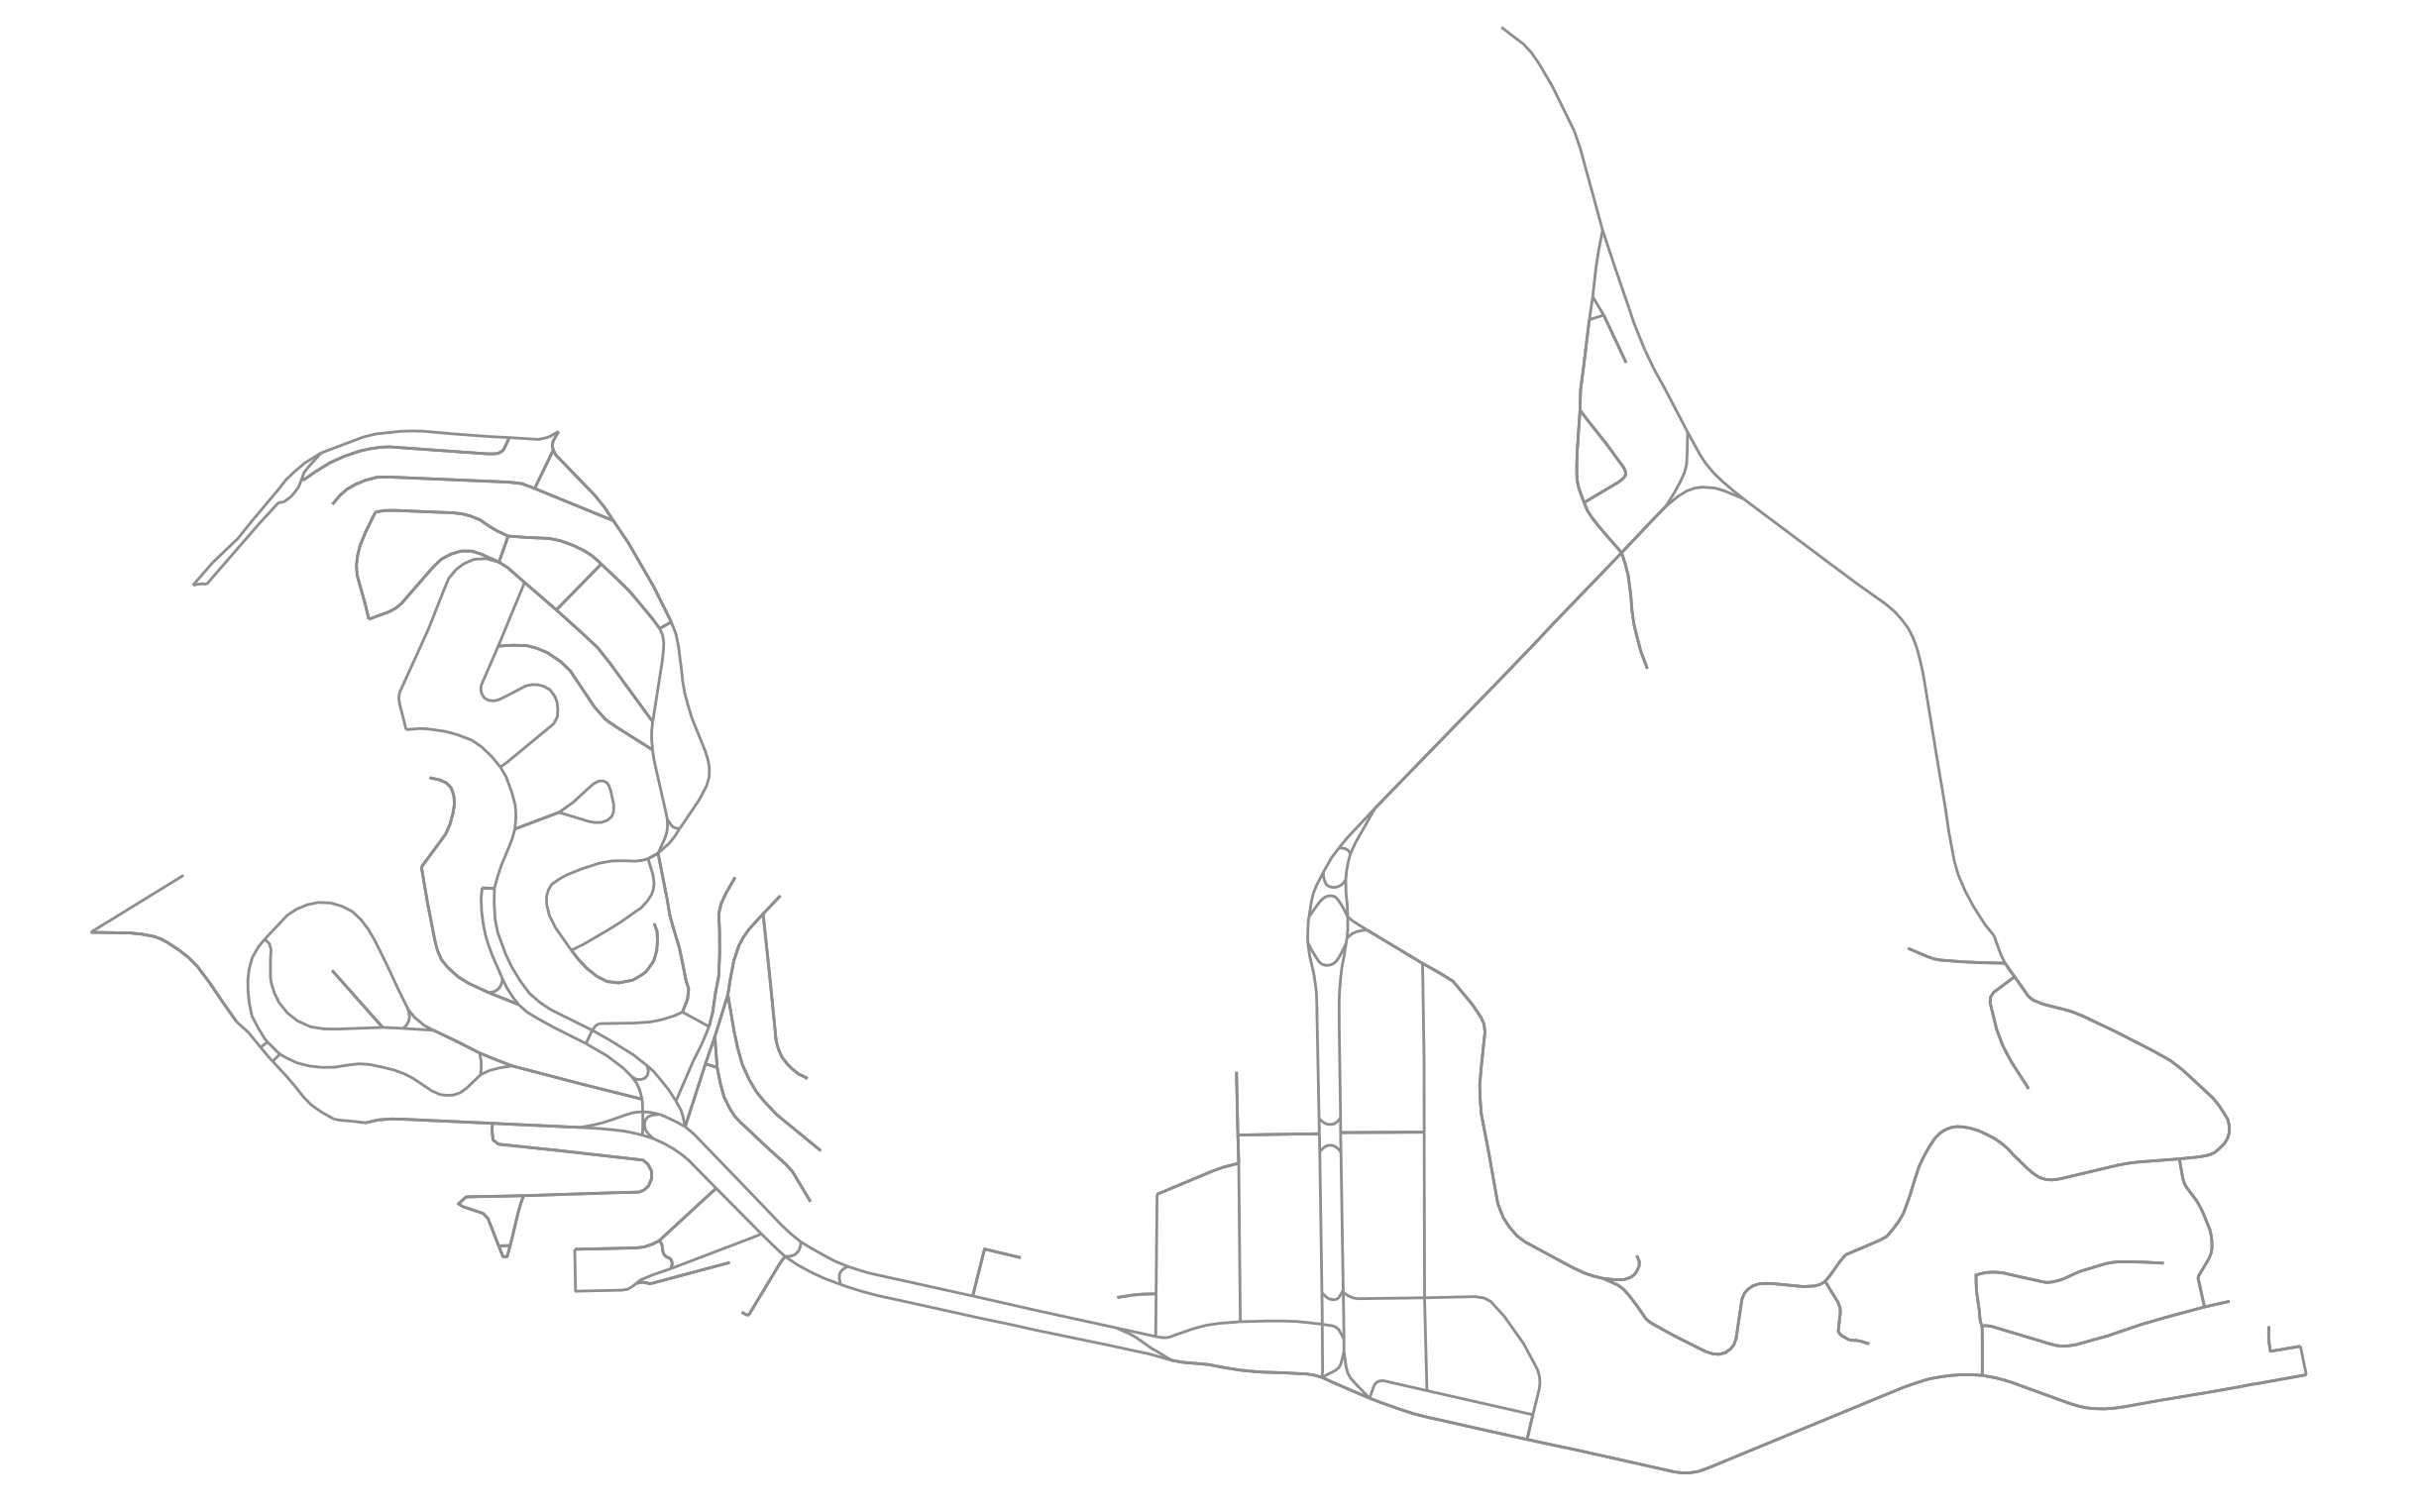
\includegraphics[width=\textwidth]{visualizacao_inicial}
    \caption{Visualização inicial das ruas do bairro de Ondina.}
    \label{fig:ondina_ruas}
\end{figure}

\subsection{Processamento e Construção do Grafo}

Após a extração dos dados, foi realizado o mapeamento para um grafo. Nesta etapa, os nós foram associados aos pontos geográficos, enquanto as arestas representaram as conexões entre eles, sendo atribuído um peso correspondente à distância entre os pontos. A Figura~\ref{fig:ondina_grafo_bruto} mostra a visualização das ruas com os vértices associados.

\begin{figure}[H]
    \centering
    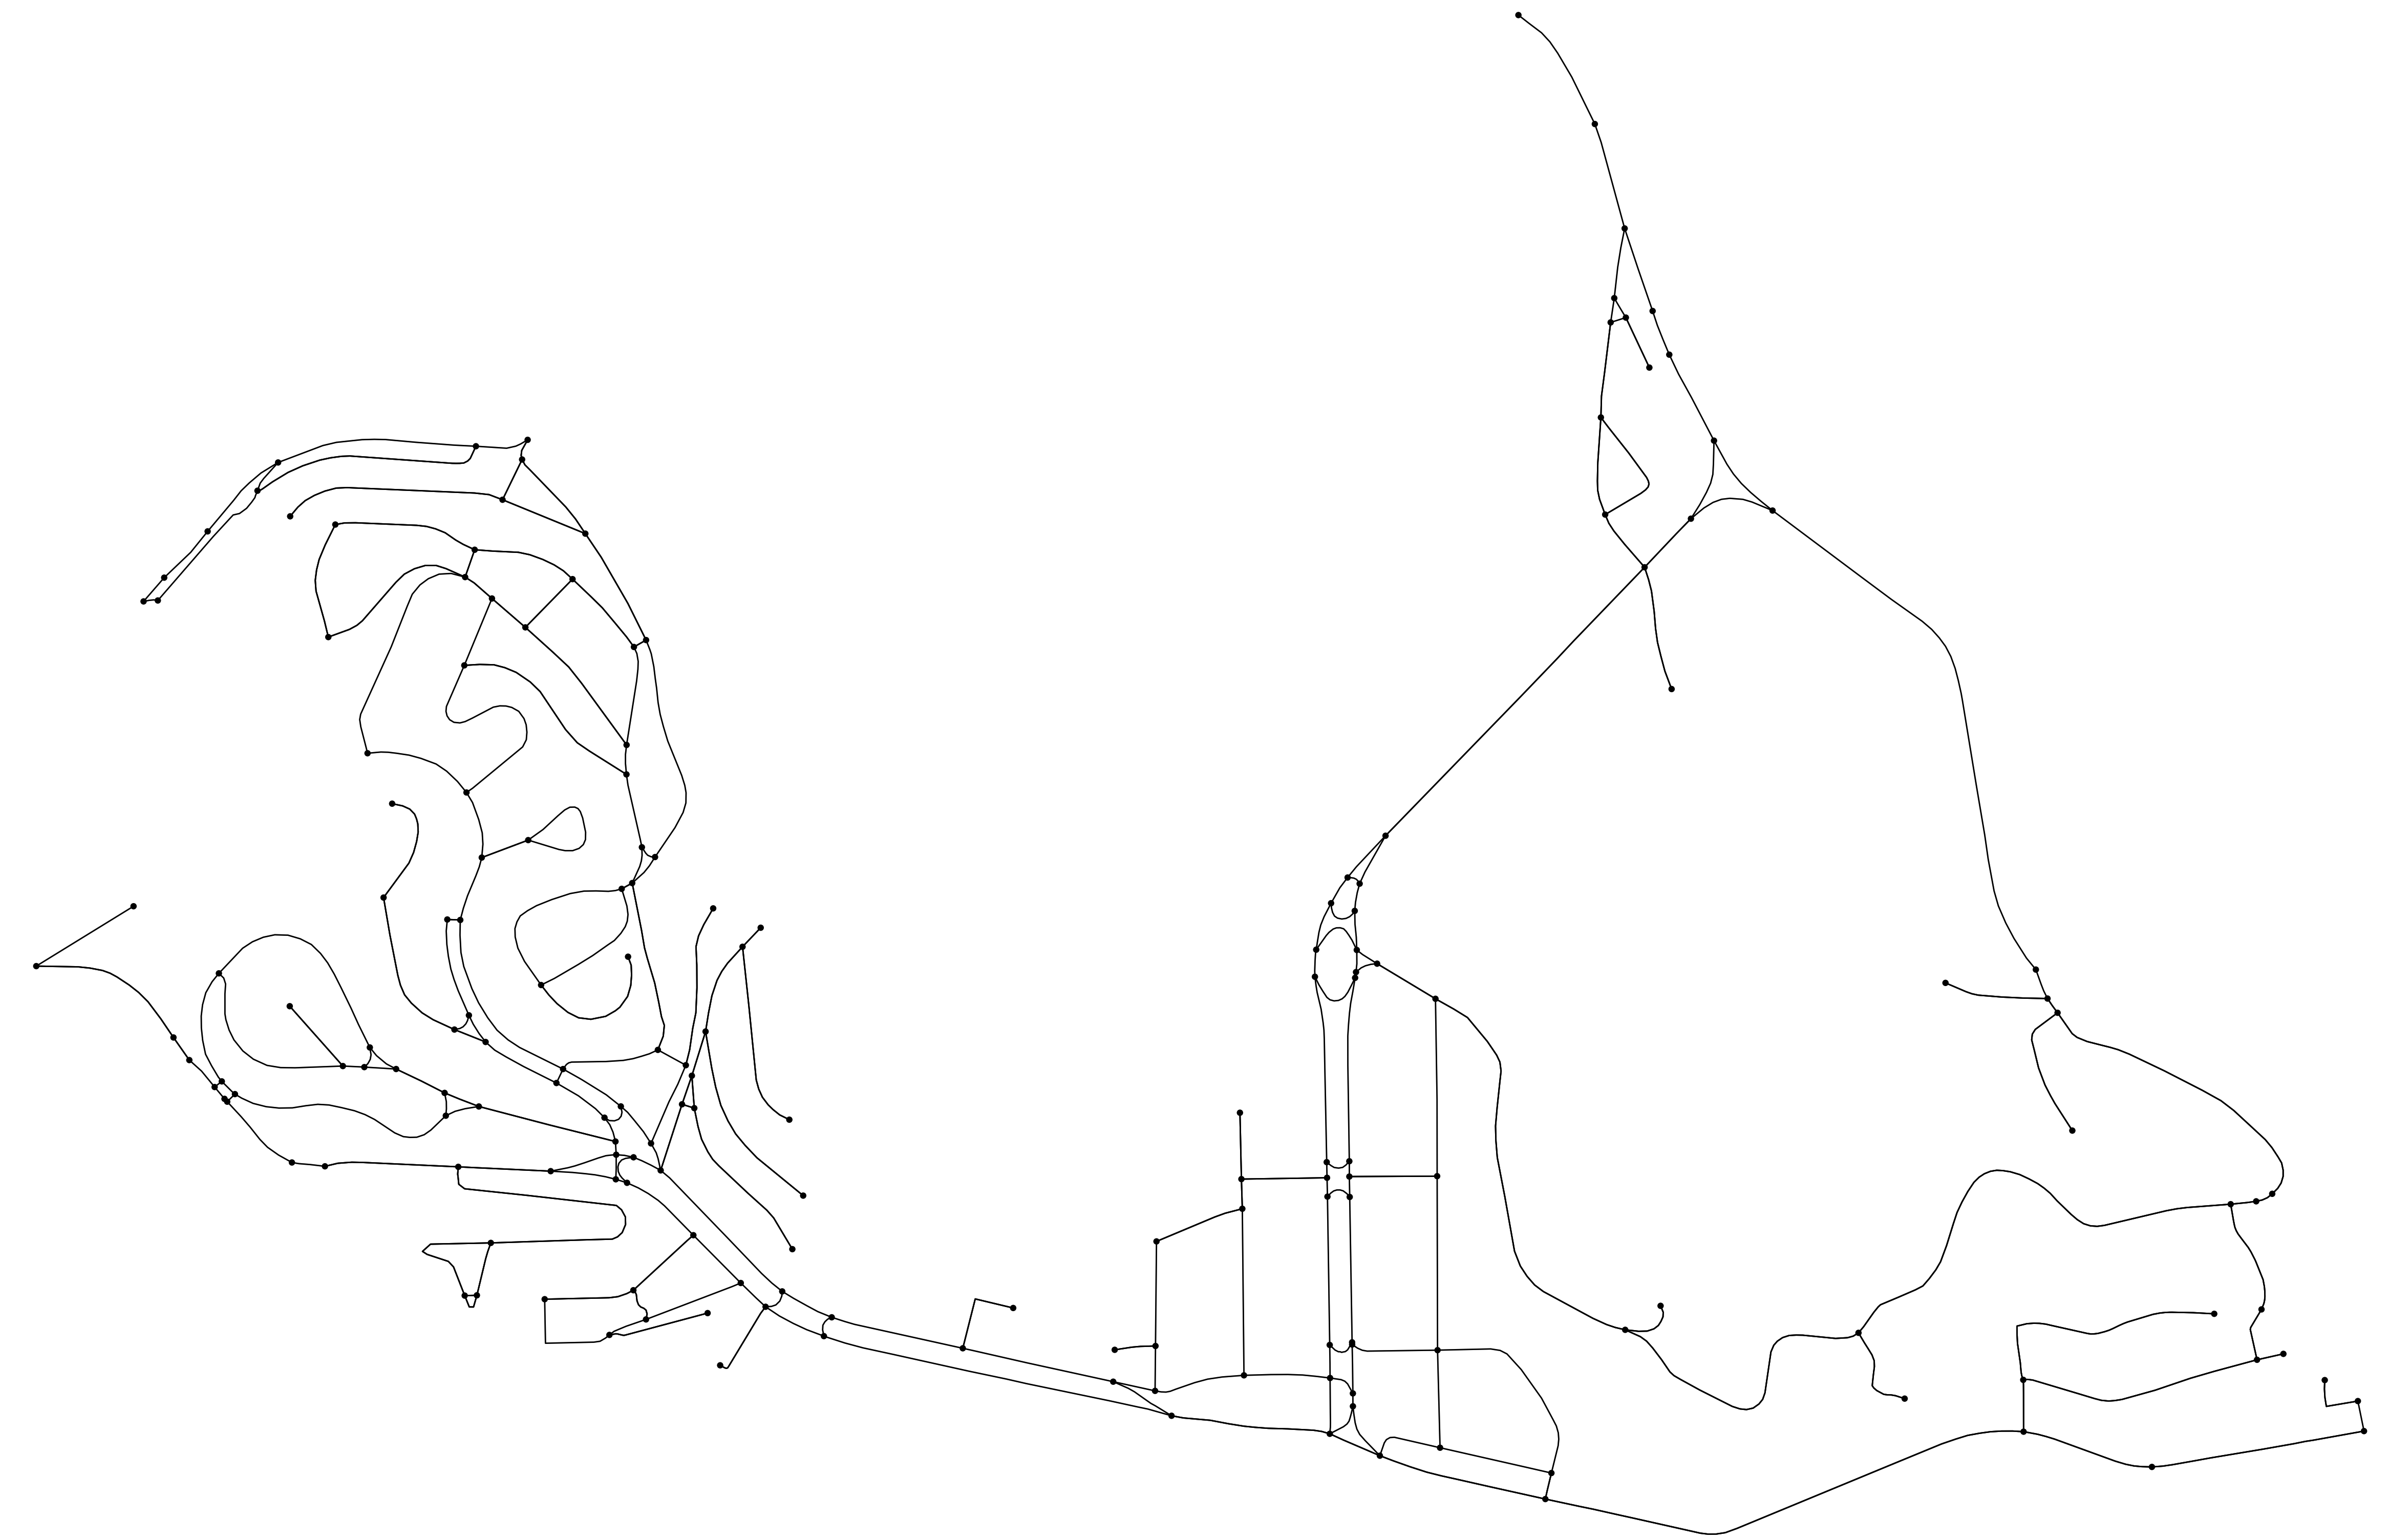
\includegraphics[width=\textwidth]{ondina_grafo_bruto}
    \caption{Visualização das ruas do bairro de Ondina com os vértices associados.}
    \label{fig:ondina_grafo_bruto}
\end{figure}

\subsection{Simplificação do Grafo}

Para adequar o grafo ao problema em análise, foi realizada uma simplificação que assumiu a existência de um campo de visão claro entre os nós conectados por uma aresta. Esta suposição eliminou obstáculos visuais e permitiu modelar de forma idealizada o problema, mantendo apenas os elementos essenciais para a análise.

O resultado do grafo simplificado é apresentado na Figura~\ref{fig:ondina_grafo_simplificado}, mostrando a estrutura final com as simplificações implementadas.

\begin{figure}[H]
    \centering
    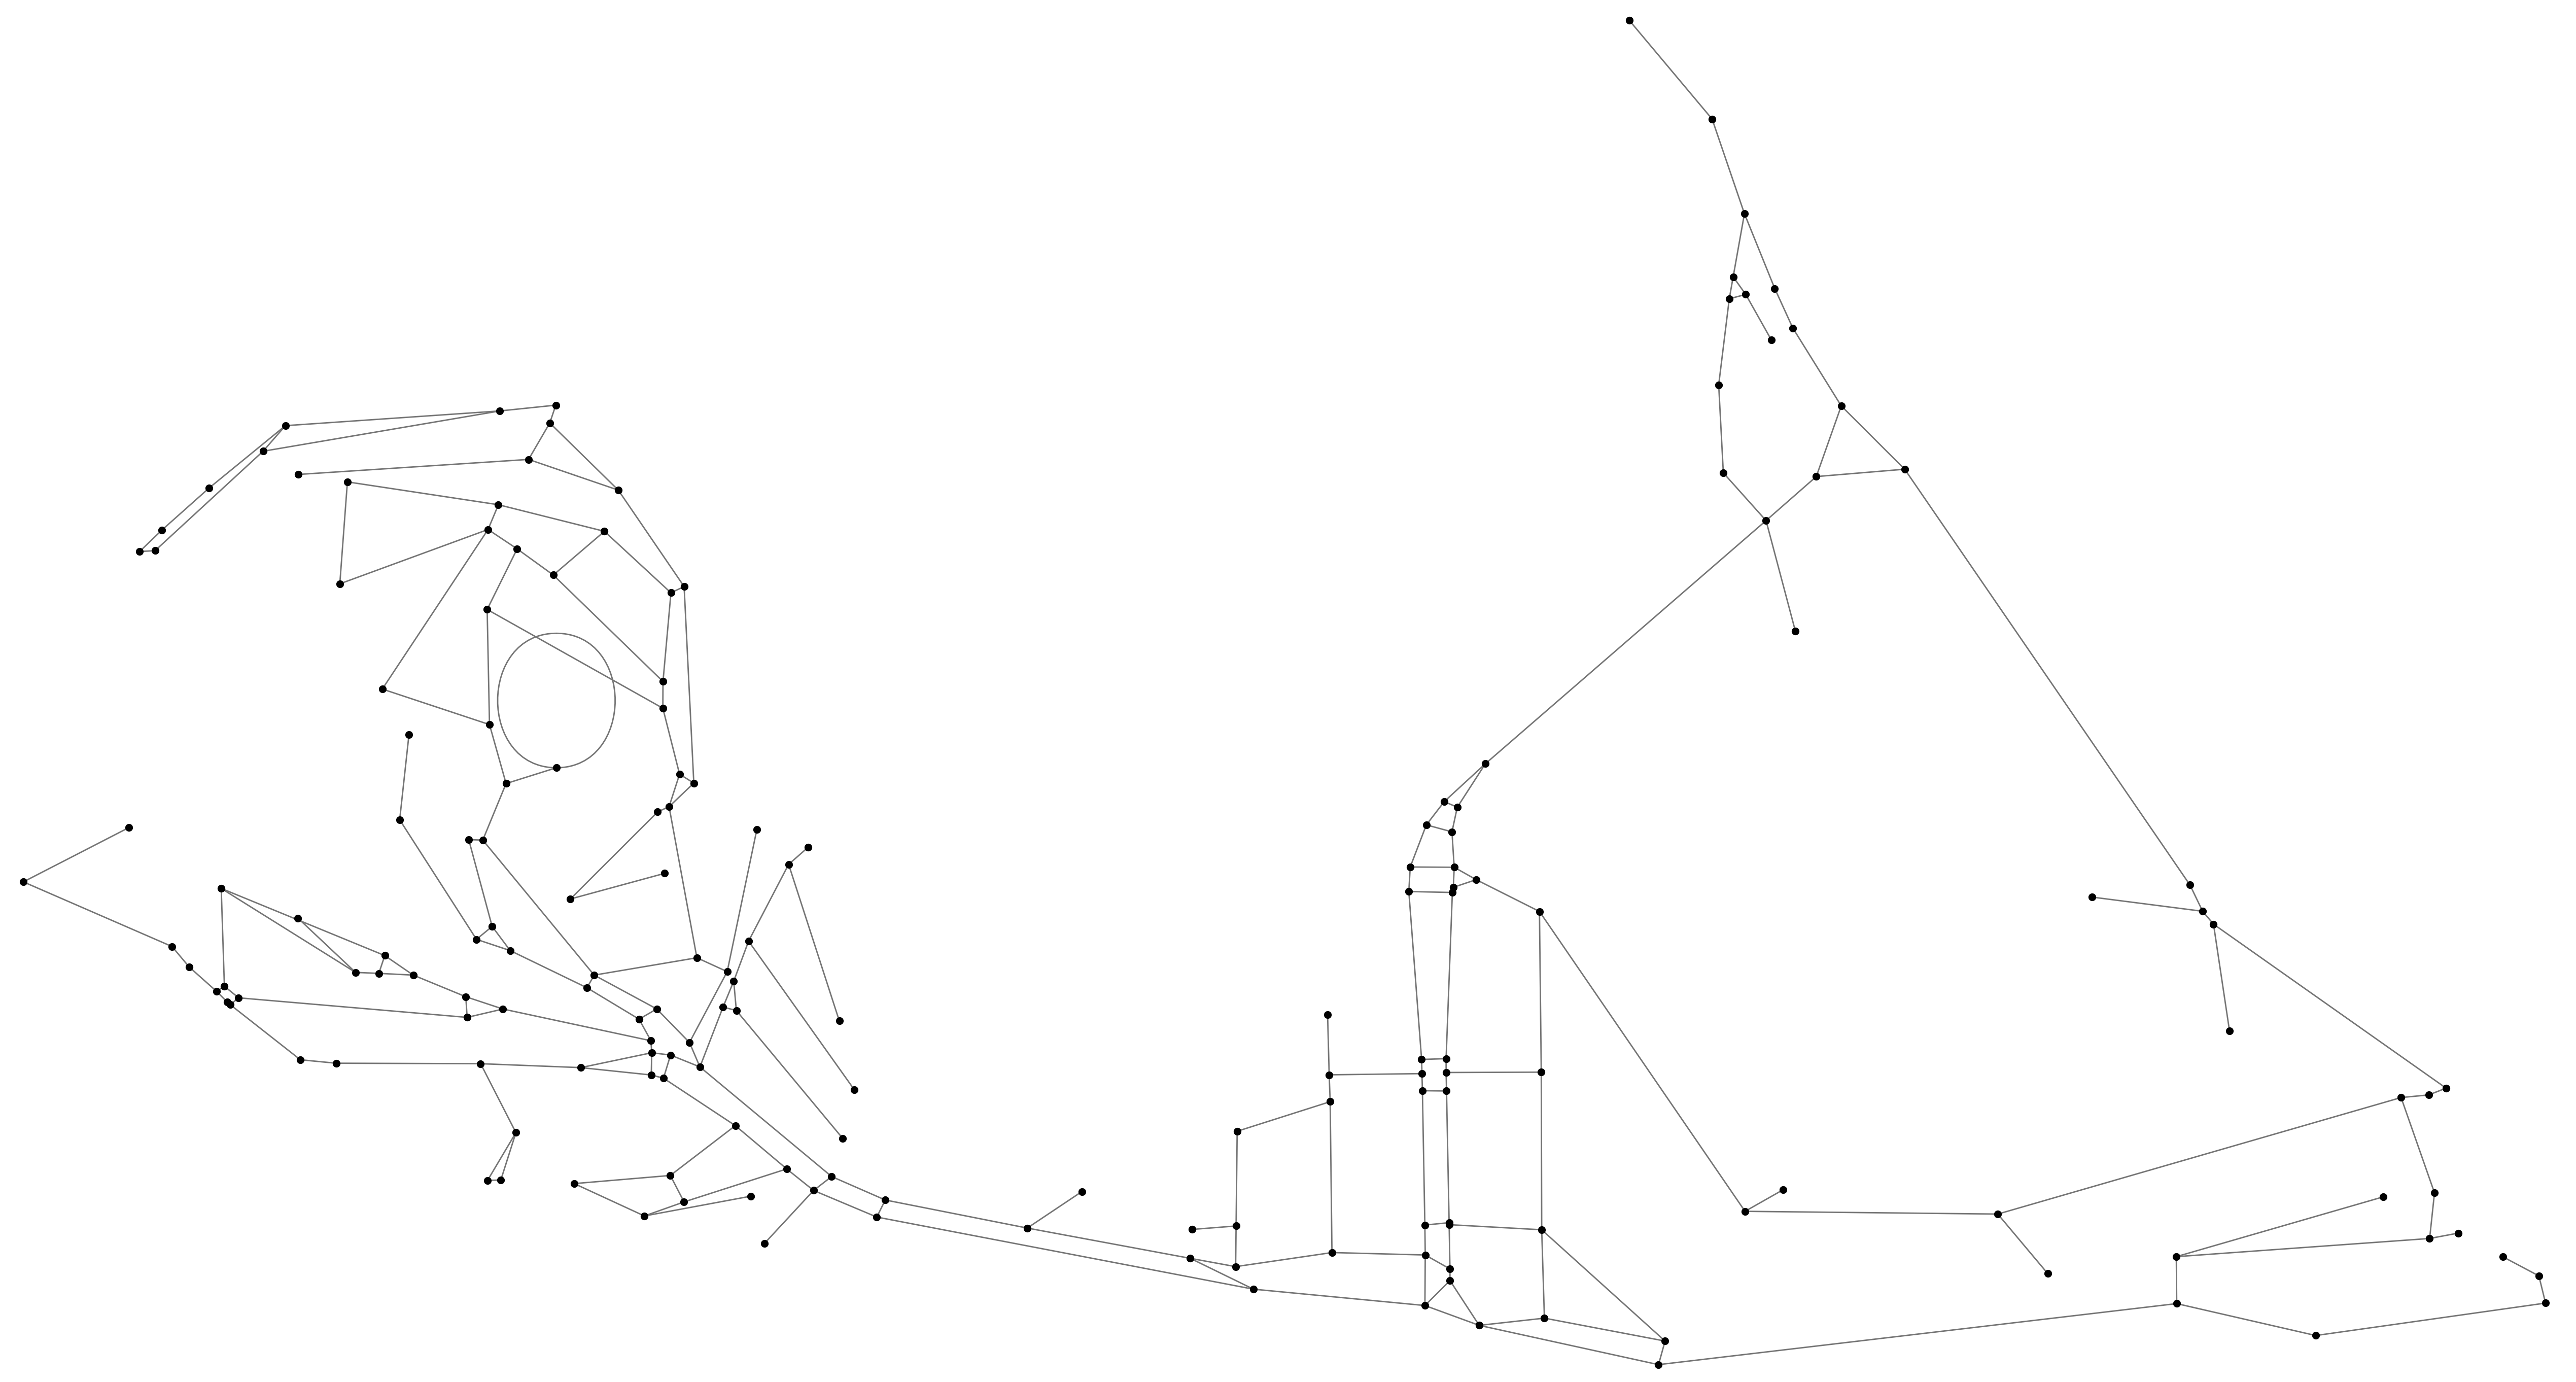
\includegraphics[width=\textwidth]{ondina_grafo_simplificado}
    \caption{Visualização do grafo simplificado do bairro de Ondina.}
    \label{fig:ondina_grafo_simplificado}
\end{figure}

\subsection{Discussão}

A simplificação realizada, ao assumir a existência de campo de visão claro entre os nós, possibilitou o uso do grafo para aplicações práticas no problema em análise. Essa abordagem é particularmente útil em cenários que envolvem monitoramento ou comunicação direta, como a análise de cobertura por câmeras, onde barreiras visuais poderiam ser tratadas como elementos externos ao modelo principal.

O processo de extração, construção e simplificação do grafo demonstra como é possível transformar dados geográficos brutos em representações abstratas otimizadas para resolver problemas específicos. A estrutura final do grafo oferece um modelo compacto e eficiente, adequado para o estudo da cobertura de vértices no contexto urbano de Ondina.

\subsection{Estrutura do Grafo}

O grafo é definido como um conjunto de \textbf{nós} e \textbf{arestas}, organizados da seguinte forma:

\begin{itemize}
    \item \textbf{Nós (Nodes):}
    Cada nó representa um ponto no mapa, definido por suas coordenadas geográficas:
    \begin{itemize}
        \item \texttt{id}: Identificador único do nó.
        \item \texttt{lat}: Latitude do ponto.
        \item \texttt{lon}: Longitude do ponto.
    \end{itemize}
    Exemplo de definição de nós:
\begin{verbatim}
{
  "id": 0,
  "lat": -13.000871,
  "lon": -38.5054976
},
{
  "id": 1,
  "lat": -13.0016275,
  "lon": -38.5057271
}
\end{verbatim}

    \item \textbf{Arestas (Edges):}
    As arestas conectam dois nós, representando ruas ou trechos que ligam os pontos geográficos. Cada aresta é caracterizada por:
    \begin{itemize}
        \item \texttt{source}: Identificador do nó de origem.
        \item \texttt{target}: Identificador do nó de destino.
        \item \texttt{weight}: Peso da aresta, que pode ser interpretado como a distância entre os dois pontos.
        \item \texttt{name}: Nome da rua ou caminho.
    \end{itemize}
    Exemplo de definição de arestas:
\begin{verbatim}
{
  "source": 0,
  "target": 3,
  "weight": 99.5182593770244,
  "name": "Avenida Anita Garibaldi"
},
{
  "source": 1,
  "target": 3,
  "weight": 96.76899596360965,
  "name": "Avenida Milton Santos"
}
\end{verbatim}
    \item \textbf{Metadados:}
    O grafo também inclui informações descritivas adicionais, como:
    \begin{itemize}
        \item \texttt{name}: Nome do grafo, neste caso, "Grafo de Ondina".
        \item \texttt{description}: Descrição geral, como "Grafo das ruas do bairro de Ondina, Salvador".
        \item \texttt{source}: Fonte dos dados, como "OpenStreetMap".
    \end{itemize}
\end{itemize}

\chapter{Solução Algorítmica}

\section{Pseudo-Código e Algoritmo Utilizado}

\subsection{Complexidade Computacional}

\subsubsection{Problema de Localização com Cobertura Completa}
O problema de encontrar o número mínimo de câmeras para cobrir todos os vértices é uma variação do problema de cobertura de conjuntos, que é um problema \textbf{NP-Difícil}. Isso significa que não existe um algoritmo conhecido que resolva esse problema em tempo polinomial para todos os casos. A complexidade computacional exata depende do tamanho da instância do problema, que é influenciado pelo número de vértices (locais potenciais para câmeras) e arestas (conexões ou alcance entre vértices).

Na prática, para resolver esse tipo de problema, são utilizados algoritmos de otimização, como o CPLEX, que foi usado no artigo de Veloso et al. \cite{veloso2021localizacao}. Esses algoritmos geralmente utilizam técnicas de \textit{branch-and-bound} e \textit{programação linear inteira}, que podem encontrar a solução ótima, mas o tempo de execução pode aumentar exponencialmente com o tamanho do problema.

\subsubsection{Problema de Localização com Cobertura Máxima}
O problema de maximizar a cobertura com um número fixo de câmeras também é \textbf{NP-Difícil}. Isso significa que, assim como o problema anterior, não há garantia de encontrar a solução ótima em tempo polinomial. A complexidade também depende do número de vértices, das conexões e do número máximo de câmeras (p) que podem ser instaladas.

O uso de algoritmos como o CPLEX também se aplica a este problema, com o objetivo de encontrar a melhor solução dentro das restrições estabelecidas.

\subsubsection{Considerações Práticas}
Em ambos os casos, a complexidade computacional pode se tornar um problema para instâncias grandes. O tempo de execução dos algoritmos pode aumentar significativamente com o número de vértices. Para instâncias maiores, é recomendável utilizar técnicas de otimização mais eficientes ou heurísticas para encontrar soluções aproximadas em um tempo razoável. A escolha do algoritmo e a modelagem adequada do problema podem influenciar significativamente o tempo de execução e a qualidade da solução obtida.

\subsection{Pseudoalgoritmos}

\subsubsection{Pseudoalgoritmo para o Problema de Localização com Cobertura Completa}
\begin{enumerate}
    \item \textbf{Entrada:} Conjunto de vértices de demanda (I), conjunto de vértices de instalação (J), matrizes de adjacência (A, B, C)
    \item \textbf{Inicialização:}
    \begin{itemize}
        \item Variável \(x[j]\) (câmera instalada para direita/cima) = 0 para todo \(j\) em \(J\).
        \item Variável \(z[j]\) (câmera instalada para esquerda/baixo) = 0 para todo \(j\) em \(J\).
        \item Variável \(k[j]\) (câmera instalada para frente) = 0 para todo \(j\) em \(J\).
    \end{itemize}
    \item \textbf{Função Objetivo:} Minimizar a soma de câmeras instaladas: \(\text{minimize} \sum_{j \in J} x[j] + \sum_{j \in J} z[j] + \sum_{j \in J} k[j]\) \cite{veloso2021localizacao}.
    \item \textbf{Restrições:}
    \begin{itemize}
        \item Garantir que cada vértice de demanda seja coberto por pelo menos uma câmera: \(\forall i \in I, \sum_{j \in J} A[i][j] \cdot x[j] + \sum_{j \in J} B[i][j] \cdot z[j] + \sum_{j \in J} C[i][j] \cdot k[j] \geq 1\)
        \item As variáveis devem ser binárias: \(x[j], z[j], k[j] \in \{0, 1\}\)
    \end{itemize}
    \item \textbf{Resolver o modelo de programação linear inteira} usando CPLEX ou outro solver adequado.
    \item \textbf{Saída:} Valores de \(x[j]\), \(z[j]\) e \(k[j]\) que indicam a localização das câmeras para cobertura completa.
\end{enumerate}

\subsubsection{Pseudoalgoritmo para o Problema de Localização com Cobertura Máxima}
\begin{enumerate}
    \item \textbf{Entrada:} Conjunto de vértices de demanda (I), conjunto de vértices de instalação (J), matrizes de adjacência (A, B, C), número máximo de câmeras (p)
    \item \textbf{Inicialização:}
    \begin{itemize}
        \item Variável \(x[j]\) (câmera instalada para direita/cima) = 0 para todo \(j\) em \(J\).
        \item Variável \(z[j]\) (câmera instalada para esquerda/baixo) = 0 para todo \(j\) em \(J\).
        \item Variável \(k[j]\) (câmera instalada para frente) = 0 para todo \(j\) em \(J\).
        \item Variável \(y[i]\) (vértice \(i\) coberto) = 0 para todo \(i\) em \(I\).
        \item Vetor \(w[i]\) (peso do vértice \(i\)) = 1 para todo \(i\) em \(I\).
    \end{itemize}
    \item \textbf{Função Objetivo:} Maximizar a soma dos pesos dos vértices cobertos: \(\text{maximize} \sum_{i \in I} w[i] \cdot y[i]\)
    \item \textbf{Restrições:}
    \begin{itemize}
        \item Garantir que um vértice seja coberto apenas se houver uma câmera que o cubra: \(\forall i \in I, \sum_{j \in J} A[i][j] \cdot x[j] + \sum_{j \in J} B[i][j] \cdot z[j] + \sum_{j \in J} C[i][j] \cdot k[j] - y[i] \geq 0\)
        \item Limitar o número total de câmeras instaladas: \(\sum_{j \in J} x[j] + \sum_{j \in J} z[j] + \sum_{j \in J} k[j] \leq p\)
        \item As variáveis devem ser binárias: \(x[j], z[j], k[j], y[i] \in \{0, 1\}\)
    \end{itemize}
    \item \textbf{Resolver o modelo de programação linear inteira} usando CPLEX ou outro solver adequado.
    \item \textbf{Saída:} Valores de \(x[j]\), \(z[j]\), \(k[j]\) e \(y[i]\) que indicam a localização das câmeras e os vértices cobertos.
\end{enumerate}

\chapter{Experimentos}

\section{Metodologia}
\subsection{Instâncias}
Os dados utilizados nos experimentos foram extraídos do OpenStreetMap, representando o bairro de Ondina. Os pontos potenciais para câmeras foram identificados com base na estrutura viária. Para garantir a representatividade dos dados, diferentes cenários foram simulados, variando o número de câmeras e o alcance de cobertura, permitindo uma análise abrangente das soluções propostas.

\subsection{Parâmetros}
Os parâmetros ajustados nos experimentos incluem o alcance das câmeras e o custo associado à instalação em diferentes locais. Esses parâmetros foram cuidadosamente selecionados para refletir condições reais de implementação, considerando fatores como visibilidade, obstáculos físicos e restrições orçamentárias.

\subsection{Testes e Critérios de Análise}
Os resultados foram avaliados com base no tempo de execução, na cobertura alcançada e na eficiência dos algoritmos implementados. Critérios adicionais, como a robustez da solução em cenários de falha e a adaptabilidade a mudanças no ambiente urbano, também foram considerados. Testes de estresse foram conduzidos para avaliar o comportamento do sistema sob condições extremas, garantindo a confiabilidade das soluções em situações reais.

\section{Resultados}
Os resultados dos experimentos são apresentados em gráficos e tabelas, destacando a eficácia das soluções encontradas. A análise dos dados revelou que a abordagem heurística proposta é capaz de reduzir significativamente o número de câmeras necessárias, mantendo uma cobertura completa das áreas de interesse. Comparações com métodos tradicionais de cobertura de vértices demonstraram a superioridade da solução em termos de custo-benefício e eficiência operacional.

\subsection{Avaliação dos Resultados}
A análise dos resultados mostra que a abordagem proposta é eficaz na redução do número de câmeras necessárias, mantendo uma cobertura completa das áreas de interesse. Além disso, a flexibilidade do algoritmo permite ajustes rápidos em resposta a mudanças no ambiente urbano, tornando-o uma solução prática e escalável para desafios de segurança pública em áreas urbanas densas.

\chapter{Considerações Finais}

\section{Conclusão}
O projeto demonstrou a aplicabilidade da teoria dos grafos na solução de problemas reais de segurança pública. A abordagem de cobertura de vértices mostrou-se eficiente e prática, oferecendo uma solução otimizada para o posicionamento de câmeras no bairro de Ondina.

%-------------Bibliografia------------------
\newpage
\renewcommand{\refname}{Referências Bibliográficas}
\addcontentsline{toc}{chapter}{Referências Bibliográficas}
\bibliography{Bibliografia}
\nocite{*}

\end{document}